\documentclass[a1paper,portrait,fontscale=0.4]{baposter}

\usepackage{relsize}
\usepackage{url}

\graphicspath{{images/}}

\definecolor{bordercol}{RGB}{40,40,40}
\definecolor{headercol1}{RGB}{186,215,230}
\definecolor{headercol2}{RGB}{80,80,80}
\definecolor{headerfontcol}{RGB}{0,0,0}
\definecolor{boxcolor}{RGB}{186,215,230}

\newcommand{\compresslist}{
	\setlength{\itemsep}{1pt}
	\setlength{\parskip}{0pt}
	\setlength{\parsep}{0pt}
}
\renewcommand\refname{}

%%%%%%%%%%%%%%%%%%%%%%%%%%%%%%%%%%%%%%%%%%%%%%%%%%%%%%%%%%%%%%%%%%%%%%%%%%%%%%%%%%
%%%%%%%%%%%%%%%%%%%%%%%%%%%%%%%%%%%%% START %%%%%%%%%%%%%%%%%%%%%%%%%%%%%%%%%%%%%%
%%%%%%%%%%%%%%%%%%%%%%%%%%%%%%%%%%%%%%%%%%%%%%%%%%%%%%%%%%%%%%%%%%%%%%%%%%%%%%%%%%

\begin{document}
\typeout{Poster rendering started}

%%%%%%%%%%%%%%%%%%%%%%%%%%%%%%%%%%%%%%%%%%%%%%%%%%%%%%%%%%%%%%%%%%%%%%%%%%%%%%%%%%
%%%%%%%%%%%%%%%%%%%%%%%%%%%%%%%%%%% BACKGROUND %%%%%%%%%%%%%%%%%%%%%%%%%%%%%%%%%%%
%%%%%%%%%%%%%%%%%%%%%%%%%%%%%%%%%%%%%%%%%%%%%%%%%%%%%%%%%%%%%%%%%%%%%%%%%%%%%%%%%%

\background{
	\begin{tikzpicture}[remember picture,overlay]%
	\draw (current page.north west)+(-2em,2em) node[anchor=north west]
	{
\includegraphics[height=1.1\textheight]{background}};
	\end{tikzpicture}
}
%%%%%%%%%%%%%%%%%%%%%%%%%%%%%%%%%%%%%%%%%%%%%%%%%%%%%%%%%%%%%%%%%%%%%%%%%%%%%%%%%%
%%%%%%%%%%%%%%%%%%%%%%%%%%%% General Poster Settings %%%%%%%%%%%%%%%%%%%%%%%%%%%%%
%%%%%%%%%%%%%%%%%%%%%%%%%%%%%%%%%%%%%%%%%%%%%%%%%%%%%%%%%%%%%%%%%%%%%%%%%%%%%%%%%%
\begin{poster}{
	grid=false,
	eyecatcher=true,
	borderColor=bordercol,
	headerColorOne=headercol1,
	headerColorTwo=headercol2,
	headerFontColor=headerfontcol,
	boxColorOne=boxcolor,
	headershape=roundedright,
	headerfont=\Large\sf\bf,
	textborder=rectangle,
	background=user,
	headerborder=open,
  boxshade=plain
}
%%%%%%%%%%%%%%%%%%%%%%%%%%%%%%%%%%%%%%%%%%%%%%%%%%%%%%%%%%%%%%%%%%%%%%%%%%%%%%%%%%
%%%%%%%%%%%%%%%%%%%%%%%%%%%%%%%%%%%% Top Left %%%%%%%.%%%%%%%%%%%%%%%%%%%%%%%%%%%%
%%%%%%%%%%%%%%%%%%%%%%%%%%%%%%%%%%%%%%%%%%%%%%%%%%%%%%%%%%%%%%%%%%%%%%%%%%%%%%%%%%
{
	\begin{minipage}[t][3cm][t]{3cm}\centering
	\vfill
	
\includegraphics[width=2.5cm]{Octave}
	\vfill
	\vfill
	\end{minipage}
}
%%%%%%%%%%%%%%%%%%%%%%%%%%%%%%%%%%%%%%%%%%%%%%%%%%%%%%%%%%%%%%%%%%%%%%%%%%%%%%%%%%
%%%%%%%%%%%%%%%%%%%%%%%%%%%%%%% Title and Subtitle %%%%%%%%%%%%%%%%%%%%%%%%%%%%%%%
%%%%%%%%%%%%%%%%%%%%%%%%%%%%%%%%%%%%%%%%%%%%%%%%%%%%%%%%%%%%%%%%%%%%%%%%%%%%%%%%%%
{\sf\bf
	Pitch Correction \\ \large\it of Digital Audio
}
%%%%%%%%%%%%%%%%%%%%%%%%%%%%%%%%%%%%%%%%%%%%%%%%%%%%%%%%%%%%%%%%%%%%%%%%%%%%%%%%%%
%%%%%%%%%%%%%%%%%%%%%%%%%%%%%%%%%%%% Sub Info %%%%%%%%%%%%%%%%%%%%%%%%%%%%%%%%%%%%
%%%%%%%%%%%%%%%%%%%%%%%%%%%%%%%%%%%%%%%%%%%%%%%%%%%%%%%%%%%%%%%%%%%%%%%%%%%%%%%%%%
{
	{\smaller\smaller 
	\vspace{1em} Walter Smuts\\
	Electrical and Computer Engineering\\
	smuts.walter@gmail.com}
}
%%%%%%%%%%%%%%%%%%%%%%%%%%%%%%%%%%%%%%%%%%%%%%%%%%%%%%%%%%%%%%%%%%%%%%%%%%%%%%%%%%
%%%%%%%%%%%%%%%%%%%%%%%%%%%%%%%%%%% Top Right %%%%%%%%%%%%%%%%%%%%%%%%%%%%%%%%%%%%
%%%%%%%%%%%%%%%%%%%%%%%%%%%%%%%%%%%%%%%%%%%%%%%%%%%%%%%%%%%%%%%%%%%%%%%%%%%%%%%%%%
{
	
\includegraphics[width=3cm]{UCT-Transparent}
}

\headerbox{Introduction}{name=Introduction,column=0,row=0}{
}

\headerbox{Pitch Detection}{name=Detection,column=0,below=Introduction}{
}

\headerbox{Pitch Shifting}{name=Shifting,column=0,below=Detection}{
}

\headerbox{References}{name=References,column=0,below=Shifting,above=bottom}{
\vspace{-3mm}
\footnotesize
\bibliography{references}{}
\bibliographystyle{ieeetr}
}

\headerbox{Basic Structure}{name=Structure,span=2,column=1,row=0}{

This flow diagram shows the basic structure of the pitch correction system. Each
block represents a module and the arrows between the modules represents the data
flow. This structure is a simplification of the structures found in the
AutoTalent\cite{Autotalent} website and the Smule patent\cite{SmulePatent}.

\vspace{3mm}
\centering
\setlength{\fboxsep}{0mm}
\fbox{\hspace{-2.5mm}
\setlength{\fboxsep}{5mm}
\colorbox{white}{
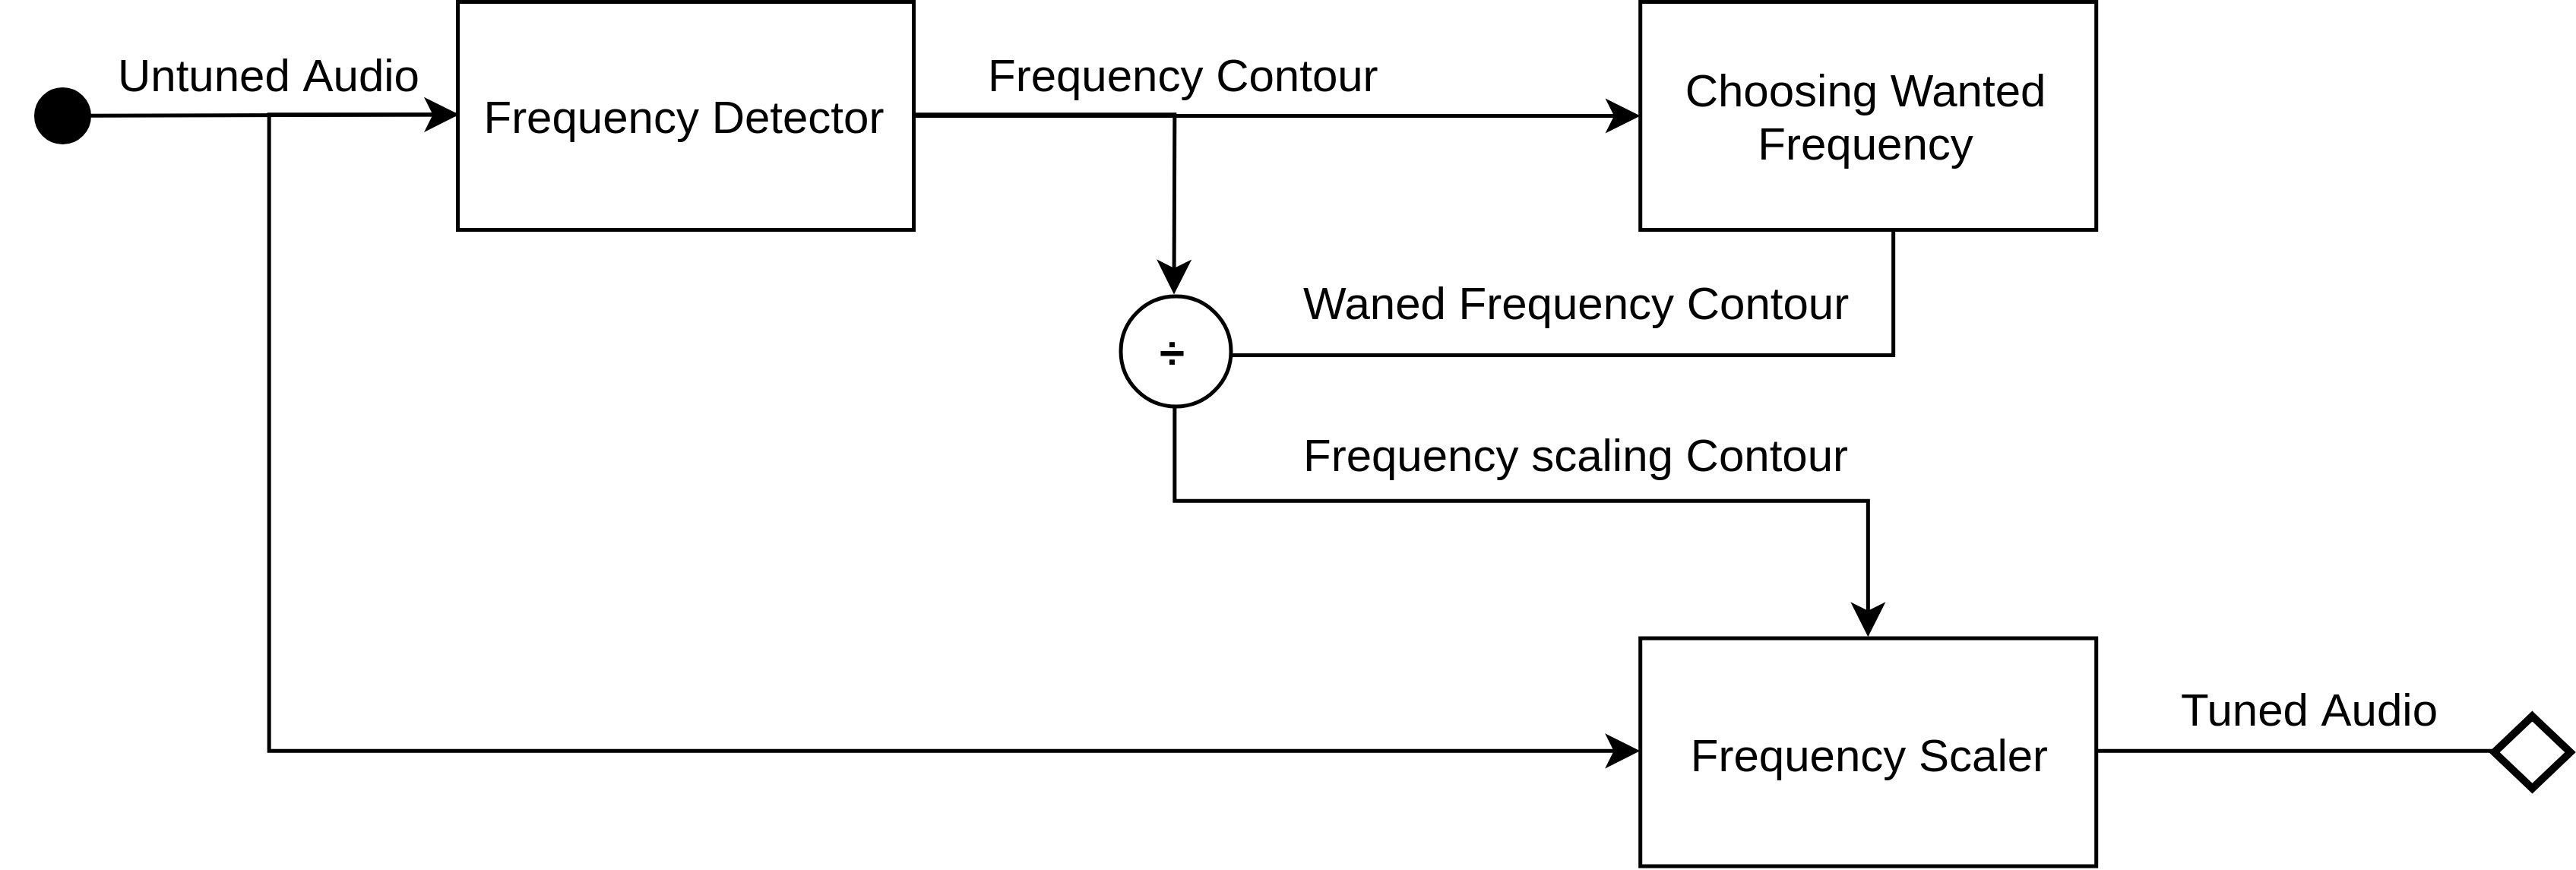
\includegraphics[width=0.925\textwidth]{PitchCorrectorFlowDiagram}
\hspace{-2.2mm}
}
\hspace{-2.2mm}
}

}

\headerbox{Pitch Detector Robustness}{name=Robustness,span=2,below=Structure,column=1,row=0}{

To measure the robustness of the pitch detector, a test was devised to see how
much white noise can be added before the pitch detector started producing large
errors. Below is a graph showing the mean squared pitch error vs added white noise
for the zero crossing method approach.

\centering
\setlength{\fboxsep}{0pt}
\fbox{\hspace{-1mm}
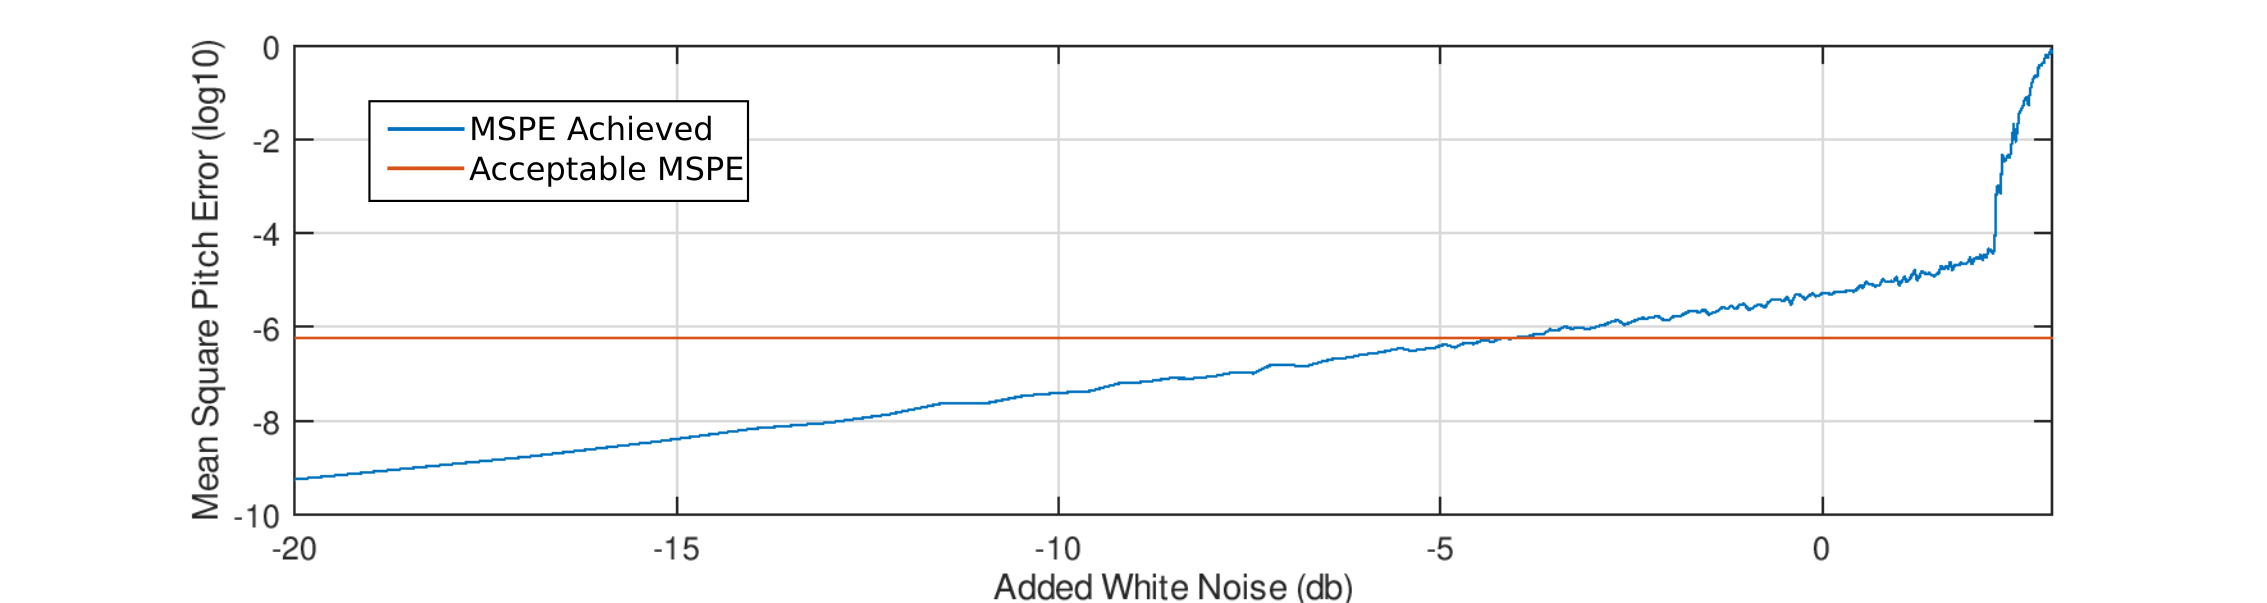
\includegraphics[width=0.99\textwidth]{NoiseRobustnessZCM}
\hspace{-1mm}}
}

\headerbox{Final Result}{name=FinalResult,span=2,below=Robustness,above=bottom,column=1}{

Below is a graph of what the final pitch correction system achieved when it was
presented with a real vocal recording. It shows the pitch contour plots of a
person singing a folk-tune ``Hansie Slim'', recorded on a laptop microphone. The
original pitch contour is shown in blue.

\setlength{\fboxsep}{0pt}
\fbox{\hspace{-1mm}
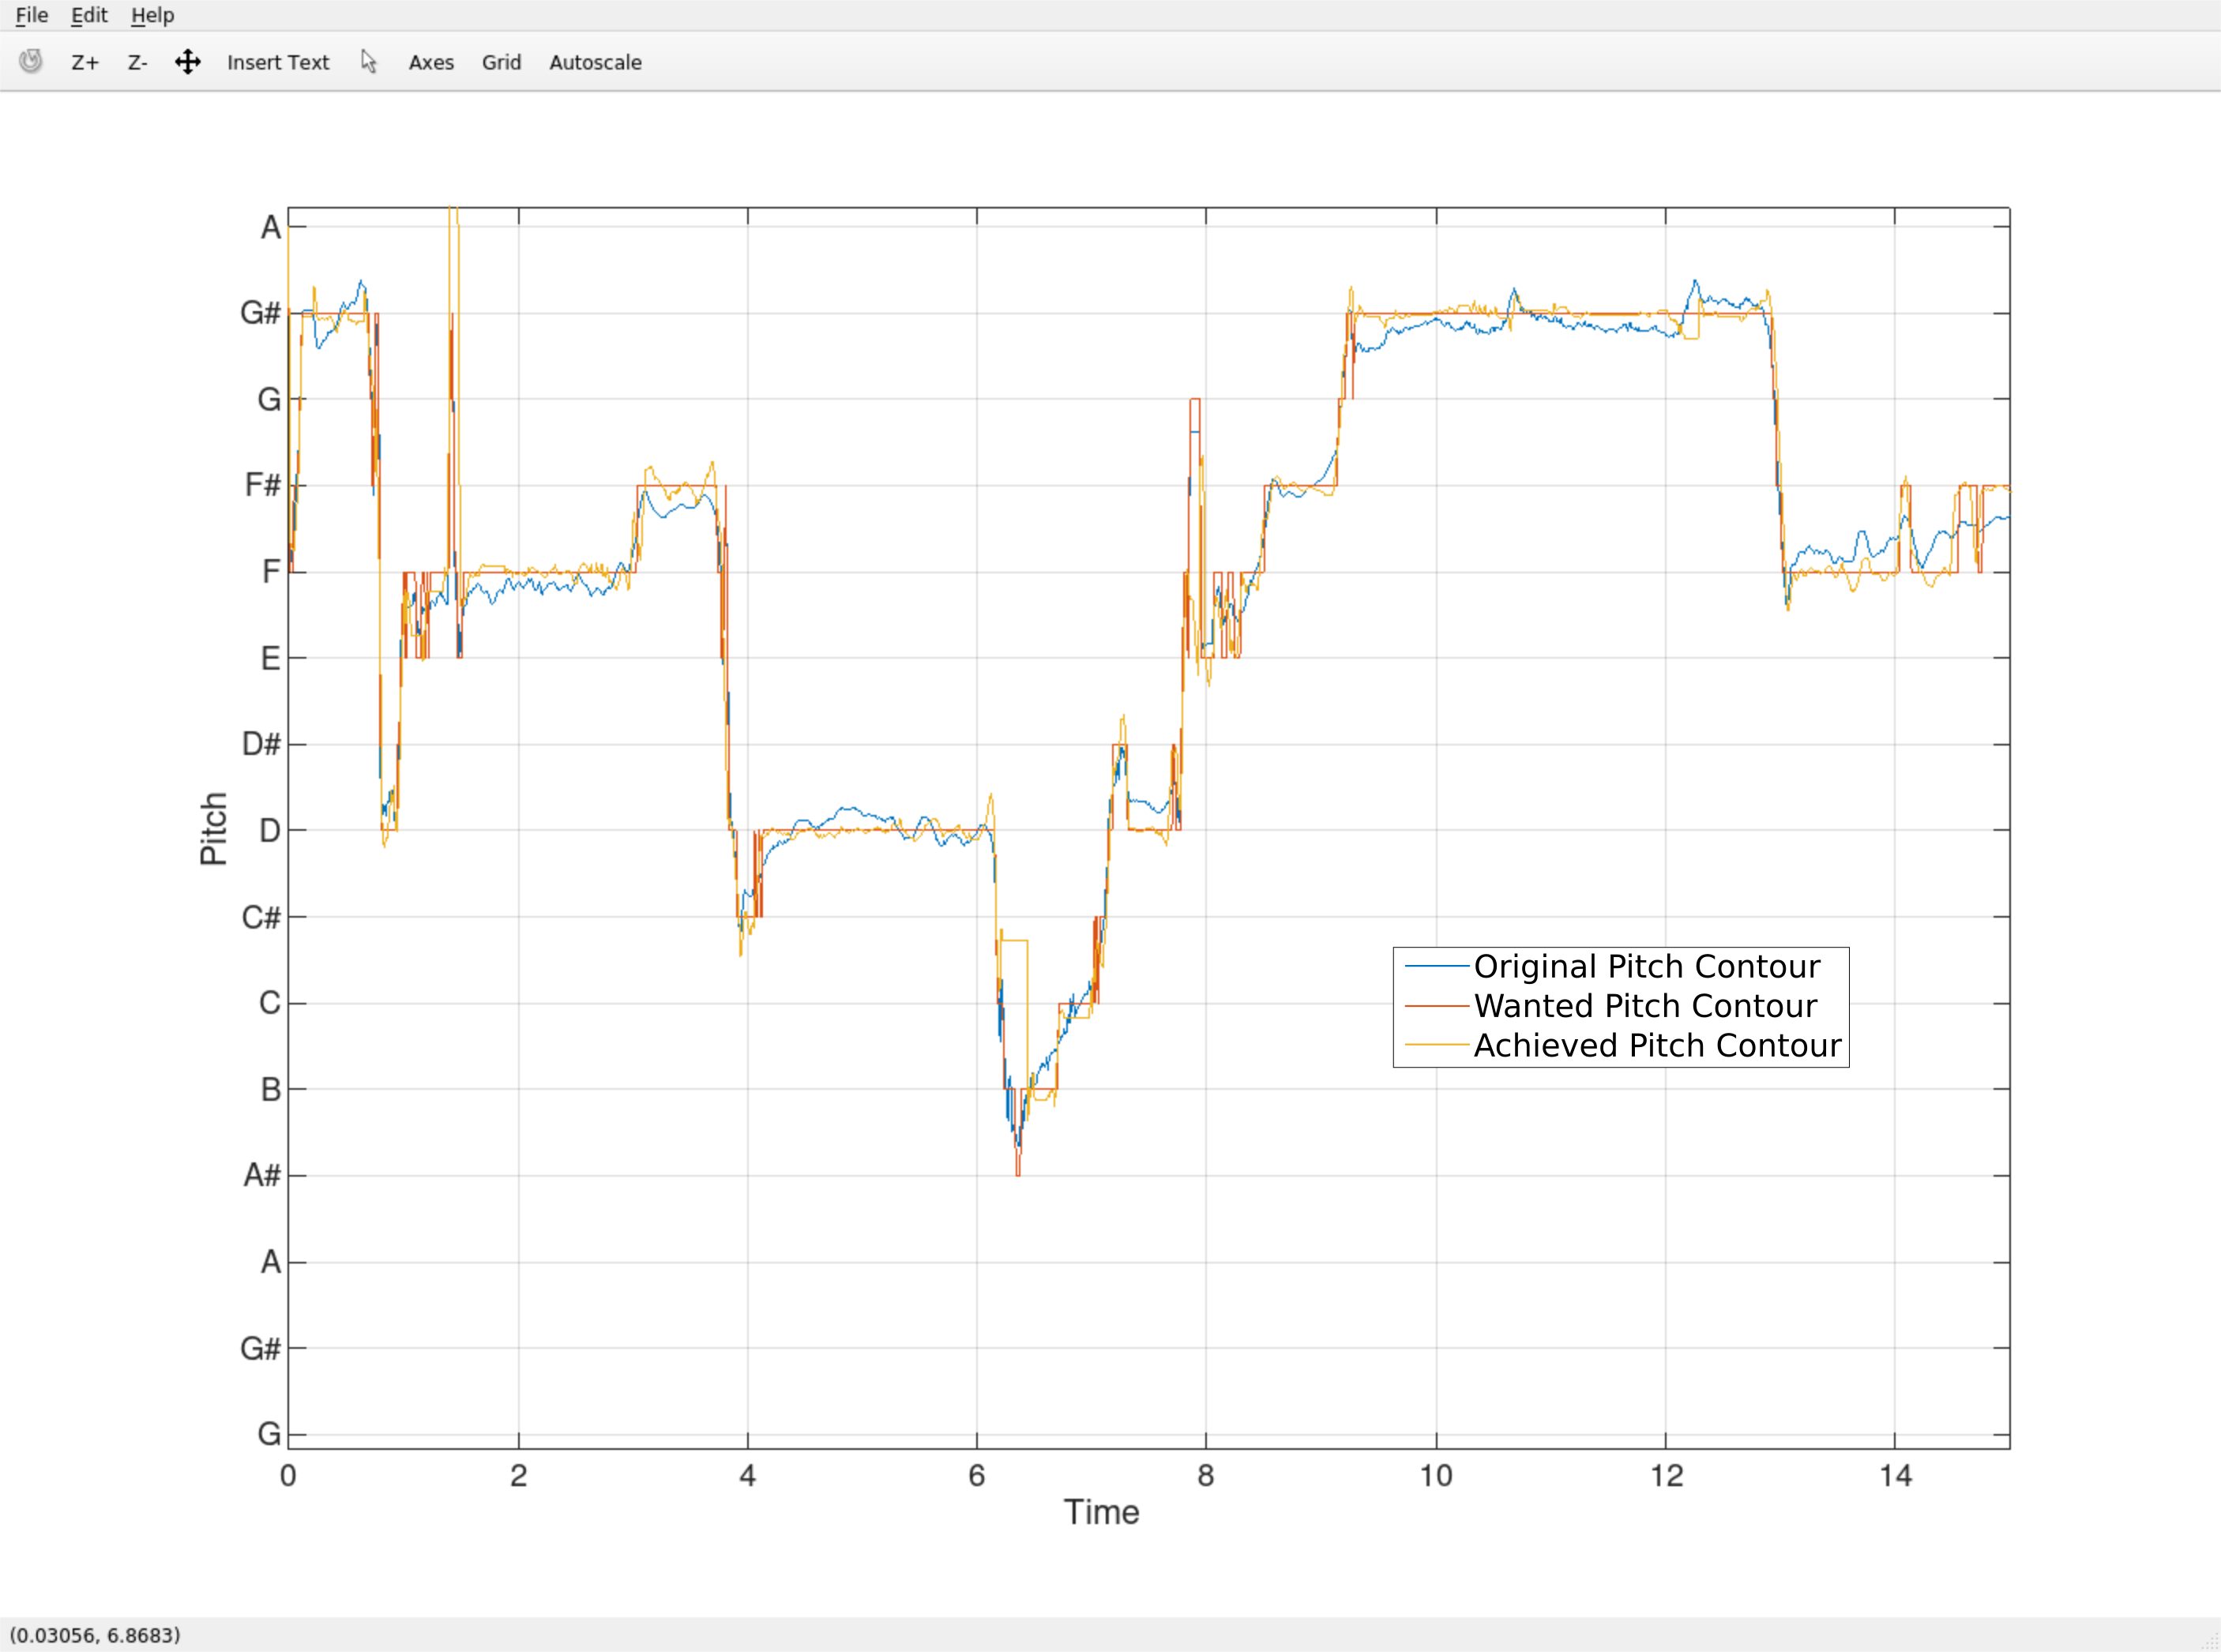
\includegraphics[width=\textwidth,clip,trim={3cm 1.5cm 3cm 3cm}]{LiveDemo}
\hspace{-1mm}}

From this graph it can be seen that the pitch contour after the correction effect
has been applied(red), seems to ``track'' the wanted pitch contour(yellow). This
tracking is akin to a more in tune recording.

}

\end{poster}
\end{document}
